\section{Proving On-Stack Replacement Sound}

On-stack Replacement is employed in modern adaptive compilation systems to dynamically switch between different versions of a function depending on program's run-time state. Traditionally, code optimizers are responsible for marking the points where such transitions can take place, and generating required meta-data or ad-hoc code to get the program state to a correct resumption point. OSR is usually at the core of large and complex JIT compilers employed by popular production virtual machines. Indeed, the engineering effort to integrate this technique in a language runtime can be daunting, making it rarely accessible to the research community.

\paragraph*{Contributions.} In this thesis we investigate how to provide VM builders with a rich ``menu'' of possible program points where OSR can safely occur, relieving code optimizers from the burden of generating all the required machinery to realign the program state during an OSR transition.

To capture OSR in its full generality, we define a notion of {\em multi-program}, which is a collection of different versions of a program along with support to dynamically transfer execution between them. Execution in a multi-program starts from a designated base version. At any time, an oracle decides whether execution should continue in the current version, or an OSR should divert it to a different version, modeling any conceivable OSR-firing strategy. One of the goals of our work is to characterize sufficient conditions for a multi-program to be {\em deterministic}, yielding the same result regardless of the oracle's decisions. This captures the intuitive idea that any sequence of OSR transitions is {\em correct} if it does not alter the intended semantics of a program.

We distill the essence of OSR to a simple imperative calculus with an operational semantics. Using program bisimulation, we prove that an OSR can correctly divert execution from one program version to the other if they are {\em live-variable bisimilar}, i.e., the live variables they have in common at any corresponding execution states are equal. As prominent examples of how bisimulation can be used to prove this property, we consider classic optimizations that eliminate or move code around, such as dead code elimination, constant propagation, and code hoisting. We show how to construct OSR machinery by devising an algorithm that automatically generates compensation code to reconstruct the values of variables that are live in the OSR target, but not in the source.

% !TEX root = thesis.tex

\begin{figure}[b]
\vspace{-2mm}
\centering
\begin{minipage}{0.63\textwidth}
\noindent
\begin{small}
$
\begin{array}{rcl}
\texttt{$Instr$} & ::= & \hphantom{\texttt{| }}\texttt{$Var$ := $Expr$} \\
& & \texttt{| if ( $Expr$ ) goto $Num$} \\
& & \texttt{| goto $Num$} \\
& & \texttt{| skip} \\
& & \texttt{| abort} \\
& & \texttt{| in $Var\cdots Var$} \\ 
& & \texttt{| out $Var\cdots Var$} \\
\texttt{ $Expr$ } & ::= & \texttt{$Num$ | $Var$ | $Expr$ + $Expr$ | $\ldots$ } \\
\texttt{ $Var$ } & ::= & \texttt{X | Y | Z | $\ldots$} \\
\texttt{ $Num$ } & ::= & \texttt{$\ldots$ | -2 | -1 | 0 | 1 | 2 | $\ldots$} \\
\end{array}
$
\end{small}
\end{minipage}
\caption{\label{fig:osr-program-syntax}Program Syntax}
\end{figure}

\subsection{Language Syntax and Semantics}
\label{ss:osr-language-framework}
Our discussion is based on a minimal imperative language whose syntax is reported \ifauthorea{below}{in \myfigure\ref{fig:osr-program-syntax}}. In this section we introduce some basic definitions used in our representation of programs, and provide a big-step semantics for the language.
%Our discussion is based on a minimal imperative programming language whose syntax is reported \ifauthorea{below}{in \myfigure\ref{fig:osr-program-syntax}}. In this section we introduce some basic definitions used in our representation of programs, and provide a big-step semantics for the language.

%\subsection{Language Framework}

%In this section we introduce some basic definitions used in our representation of programs and transformations. In particular, we provide a syntax and a big-step semantics for a simple imperative language, and introduce means for reasoning about program properties using computation tree logic operators and for describing program transformations through rewrite rules with side conditions.

%\subsubsection*{Program Syntax and Semantics}

%Our discussion is based on a minimal imperative programming language with instructions and expressions with the syntax \ifauthorea{below}{in \myfigure\ref{fig:osr-program-syntax}}.

\begin{definition}[Program]
\label{de:program}
A program is a sequence of instructions the form:
\vspace{-3mm}
\begin{equation*}
\pi=\langle I_1, I_2, \ldots, I_n \rangle\in Prog = \bigcup_{i=2}^{\infty} Instr^{i}
\vspace{-4mm}
\end{equation*}
where: 

\begin{itemize}[itemsep=3pt,parsep=0pt,topsep=3pt]
%\item $Instr$ is defined by the syntax of Figure~\ref{fi:program-syntax}
\item \texttt{$I_i\in Instr$} is the $i$-th instruction of the program, indexed by program point \texttt{$i\in[1,n]$}
\item \texttt{$I_1$ $=$ in $\cdots$} is the initial instruction
\item \texttt{$\forall i\in[2,n-1]:$ $I_i$ $\neq$ in $\cdots$ $\wedge$ $I_i$ $\neq$ out $\cdots$}
\item \texttt{$I_n$ $=$ out $\cdots$} is the final instruction
\end{itemize}
\end{definition}

\noindent Instruction \texttt{in}, which must appear at the beginning of a program, specifies the variables that must be defined prior to entering the program. Similarly, \texttt{out} occurs at the end and specifies the variables that are returned as output. 

\noindent By \texttt{e[x]} we indicate that \texttt{x} is a variable of expression \texttt{e}\,$\in Expr$. We also denote by $vars($\texttt{e}$)$ the set of variables that occur in expression \texttt{e}. By $|\pi|=n$ we indicate the number of instructions in $\pi=\langle I_1, I_2, \ldots, I_n \rangle$.

\begin{definition}[Memory Store]
A {\em memory store} is a total function $\sigma:Var\rightarrow \mathbb{Z}\cup\{\bot\}$ that associates integer values to defined variables, and $\bot$ to undefined variables. We denote by $\Sigma$ the set of all possible memory stores. 
\end{definition}

\noindent By $\sigma[\wx\gets v]$ we denote the same function as $\sigma$, except that $\wx$ takes value $v$. Furthermore, for any $A\subseteq Var$, $\sigma\vert_{A}$ denotes $\sigma$ restricted to the variables in $A$, i.e., $\sigma\vert_{A}(\wx)=\sigma(\texttt{x})$ if $\wx\in A$ and $\sigma\vert_{A}(\wx)=\bot$ if $\wx\not\in A$. 

\begin{definition}[Program State]
\label{de:prog-state}
The {\em state} of a program $\pi=\langle I_1, I_2, \ldots, I_n \rangle$ is described by a pair $(\sigma,l)$, where $\sigma$ is a memory store and $l\in [1,n]$ is the program point of the next instruction to be executed. We denote by $State=\Sigma\times \mathbb{N}$ the set of all possible program states.
\end{definition}

\noindent We provide a big-step semantics using the transition relation $\trans_{\pi}\:\subseteq State\times State$, which specifies how a single instruction of a program $\pi$ affects its state. Our description relies on the relation $\Downarrow\subseteq(\Sigma\times Expr)\times \mathbb{Z}$ to describe how expressions are evaluated in a given memory store.


\begin{definition}[Big-Step Transitions]
\label{de:transitions}
%For any program $\pi$, relation $\Rightarrow_{\pi}\subseteq State\times State$ is defined as follows, with meta-variables $\texttt{x}, \texttt{y}\in Var$, $\texttt{e}\in Expr$, and $\texttt{m}\in Num$:
For any program $\pi$, we define relation $\Rightarrow_{\pi}\:\subseteq State\times State$ as follows, with meta-variables $\texttt{x}, \texttt{y}\in Var$, $\texttt{e}\in Expr$, and $\texttt{m}\in Num$:

\begin{small}

% asgn
\begin{equation}
\label{eq:asgn-sem}
\frac
{I_l=\texttt{x:=e} ~~ \wedge ~~ (\sigma, \texttt{e}) \Downarrow v}
{(\sigma, l)\Rightarrow_{\pi} (\sigma[\wx\gets v], l+1)}
\end{equation}
% if (0)
\vspace{0.5mm}
\begin{equation}
\label{eq:ifz-sem}
\frac
{I_l=\texttt{if (e) goto m} ~~ \wedge ~~ (\sigma, \texttt{e}) \Downarrow 0}
{(\sigma, l)\Rightarrow_{\pi} (\sigma, l+1)}
\end{equation}
% if (!0)
\vspace{0.5mm}
\begin{equation}
\label{eq:ifnz-sem}
\frac
{I_l=\texttt{if (e) goto m} ~~ \wedge ~~ (\sigma, \texttt{e}) \Downarrow v ~~~ \wedge ~~~ v\neq 0}
{(\sigma, l)\Rightarrow_{\pi} (\sigma, \texttt{m})}
\end{equation}
% goto
\vspace{0.5mm}
\begin{equation}
\label{eq:goto-sem}
\frac
{I_l=\texttt{goto m}}
{(\sigma, l)\Rightarrow_{\pi} (\sigma, \texttt{m})}
\end{equation}
% skip
\vspace{0.5mm}
\begin{equation}
\label{eq:skip-sem}
\frac
{I_l=\texttt{skip}}
{(\sigma, l)\Rightarrow_{\pi} (\sigma, l+1)}
\end{equation}
% in
\vspace{0.5mm}
\begin{equation}
\label{eq:in-sem}
\frac
{I_1=\texttt{in x y}~\cdots ~~ \wedge ~~~ \sigma(\texttt{x})\neq\bot ~~~ \wedge ~~~ \sigma(\texttt{y})\neq\bot ~~~ \wedge ~~~ \cdots }
{(\sigma, 1)\Rightarrow_{\pi} (\sigma, 2)}
\end{equation}
% out
%\vspace{0.5mm}
\begin{equation}
\label{eq:out-sem}
\frac
{I_n=\texttt{out x y}~\cdots ~~ \wedge ~~~ \sigma(\texttt{x})\neq\bot ~~~ \wedge ~~~ \sigma(\texttt{y})\neq\bot ~~~ \wedge ~~~ \cdots }
{(\sigma, n)\Rightarrow_{\pi} (\sigma\vert_{\{\texttt{x}, \texttt{y}, \cdots\}}, n+1)}
\end{equation}

\end{small}

\end{definition}

\noindent For a transition to apply, we implicitly assume that $I_l$ is defined, i.e., $l\in[1,n]$. 
\ifx\noauthorea\undefined
Notice that we intentionally do not provide any transition rule for {\tt abort} instructions, providing explicit means to let a program have undefined semantics. This might be useful in supporting unsound speculative optimizations.
\fi

\begin{definition}[Program Semantic Function]
\label{de:program-semantics}
%The semantic function $\mysem{\pi}:\Sigma \rightarrow \Sigma$ of a program $\pi$ is defined as:
We define the semantic function $\mysem{\pi}:\Sigma \rightarrow \Sigma$ of a program $\pi$ as: 
\begin{gather*}
\forall \sigma\in\Sigma: ~~ \mysem{\pi}(\sigma)=\sigma'~~%\vert_{\{\wx\,:\,I_{n}={\tt out}~\cdots~\wx~\cdots\}} ~~ \\ 
\Longleftrightarrow ~~ (\sigma,1) \Rightarrow^{*}_{\pi} (\sigma',|\pi|+1)
\end{gather*}
where $\Rightarrow^{*}_{\pi}$ is the transitive closure of $\Rightarrow_{\pi}$.
\end{definition}

\noindent Note that a program has undefined semantics if its execution on a given store does not reach the final \texttt{out} instruction. This accounts for infinite loops, abort instructions, exceptions, and ill-defined programs or input stores. 

We define the notion of program semantic equivalence as follows:

\begin{definition}[Program Equivalence]
\label{de:semantic-equivalence}
Two programs $\pi_1$ and $\pi_2$ are {\em semantically equivalent} iff $\mysem{\pi_1}=\mysem{\pi_2}$.
\end{definition}

\noindent A notion that will be useful in proving correctness in our framework is that of a {\em trace} of a transition system:

\begin{definition}[Traces]
\label{de:exec-trace}
A {\em trace} in a transition system $(S,$ $R\subseteq S^2)$ starting from $s\in S$ is a sequence $\tau=\langle s_0,s_1,\ldots,$ $s_i,\ldots\rangle$ such that $s_0=s$ and $\forall i\ge 0:~s_i\in\tau ~ \wedge ~ s_i~R~s_{i+1}$ $\Longleftrightarrow s_{i+1}\in\tau$. By ${\cal T}_{R,s}$ we denote the system of all traces of $(S,R\subseteq S^2)$ starting from $s$. By $\tau[i]$ we denote the $i$-th state of $\tau$, i.e., $\tau[i]=s_i$. Furthermore, if trace $\tau$ is finite then $|\tau|$ denotes the index of its final state, i.e., $\tau=\langle s_0,s_1,\ldots,s_{|\tau|}\rangle$, otherwise $|\tau|=\infty$. Finally, $dom(\tau)=\{i:s_i\in\tau\}$ denotes the set of indices of states in $\tau$.
\end{definition}

\noindent Notice that since $\Rightarrow_{\pi}$ is deterministic in our language, then for any initial store $\sigma$, the system of traces ${\cal T}_{\Rightarrow_{\pi},(\sigma,1)}$ of the execution transition system $(Store,\Rightarrow_{\pi})$ contains a single trace, which we denote by $\tau_{\pi\sigma}$.

Finally, we provide a formal definition of a control flow graph, which will be useful in defining computation tree logic operators for reasoning on program properties:

\begin{definition}[Control Flow Graph]
\label{de:cfg}
%The {\em control flow graph} G for a program $\pi=\langle I_1, I_2, \ldots, I_n \rangle$ is described by a pair $(V,E)$ where $V = \{ I_1, I_2, \ldots, I_n \}$ and $E = \{(I_i, I_{i+1})\:|\: I_i \neq \textsf{abort} \wedge I_i \neq \textsf{goto m}, \!\textsf{ m}\in Num \}\;\cup\;\{(I_i, I_m)\:|\: I_i = \textsf{goto m} \vee I_i = \textsf{if (e) goto m}, \!\textsf{ m}\in Num, \!\textsf{ e}\in Expr \}$.
%The {\em control flow graph} G for a program $\pi=\langle I_1, I_2, \ldots, I_n \rangle$ is described by a tuple $\langle V, I: V\rightarrow Num, E \subseteq V\times V\rangle$ where:
The {\em control flow graph} $G$ for a program $\pi=\langle I_1, I_2, \ldots, I_n \rangle$ is described by a pair $(V, E \subseteq V\times V)$ where:
%\begin{equation*}
\begin{align*}
V &= \{ I_1, I_2, \ldots, I_n \} \\
%I(v) &= \{ i | v = I_i, v\in V\} \\
E &= \{(I_i, I_{i+1})\:|\: I_i \neq \textsf{abort} \wedge I_i \neq \textsf{goto m}, \!\textsf{ m}\in Num \} \\
&\cup\;\{(I_i, I_m)\:|\: I_i = \textsf{goto m} \vee I_i = \textsf{if (e) goto m}, \!\textsf{ m}\in Num, \!\textsf{ e}\in Expr \}.
\end{align*}
%\end{equation*}
%\noindent We also define an auxiliary function $I: V\rightarrow Num$ that returns the $i$-th index in $\pi$ of an instruction $v\in V$.
\end{definition}
% !TEX root = thesis.tex

\subsection{Program Properties and Transformations}
\label{ss:osr-reasoning-and-transformations}

In this section we present a formalism based on {\em computation tree logic} (CTL) to reason about program properties and describe program transformations through rewrite rules with side conditions~\cite{Clarke86,Lacey04,Kalvala09}.

\subsubsection*{Reasoning about Program Properties}

To analyze properties of a program, we use Boolean formulas with free meta-variables that combine facts that must hold globally or at certain points of a program. Formulas can be checked against concrete programs by a {\em model checker}. For any program $\pi$ and formula $\phi$, the checker verifies whether there exists a substitution $\theta$ that binds free meta-variables with program objects so that $\theta(\phi)$ is satisfied in $\pi$. 
In this thesis, by $\cal{A}\models \phi$ we mean that $\phi$ is true in $\cal{A}$, i.e., formula $\phi$ is satisfied by structure $\cal{A}$ (or equivalently, $\cal{A}$ models $\phi$)~\cite{Clarke86}. %We use notation $\cal{A}\models_{\theta} \phi$ as a shortcut for $\cal{A}\models \theta(\phi)$. 

\noindent Two global predicates that we will use later on are ${\tt conlit}(\wc)$, which states that an expression $\wc$ is a constant literal, and ${\tt freevar}(\wx,\we)$, which holds if and only if $\wx$ is a free variable of expression $\we$.

%To support analyses based on facts that involve finite maximal paths in the control flow graph (CFG), such as liveness and dominance, we use formulas based on {\em computation tree logic} (CTL) operators~\cite{Clarke86,Lacey04,Kalvala09}. In order to introduce these operators, we need to formalize the concept of finite maximal paths first.
To support analyses based on facts that involve finite maximal paths in the control flow graph (CFG), such as liveness and dominance, we use formulas based on CTL operators. In order to introduce these operators, we need to formalize the concept of finite maximal paths first.

\begin{definition}[Set of Complete Paths] Given a control flow graph $G=(V,E)$ and an initial node $n_0\in V$, the {\em set of complete paths} $CPaths(n_0,G)$ starting at $n_0$ consists of all finite sequences $\langle n_0,n_1,\ldots,n_k\rangle$ such that $(n_i,n_{i+1})\in E$ for all $n_i$ with $i<k$, and such that there does not exist a $n_{k+1}$ such that $(n_k,n_{k+1})\in E$.
\end{definition}

\noindent Complete paths from a specified node (i.e., instruction) are thus maximal finite sequences of connected nodes through a control flow graph from an initial point to a sink node, which in our setting is unique (unless {\tt abort} instructions are present) and corresponds to the final instruction $I_n$.

First-order CTL can be used to specify properties of nodes and paths in a CFG. In particular, temporal CTL operators can be used to express properties of some or all possible future computational paths, any one of which might be an actual path that is realized. Before formalizing the temporal operators that we are going to use in the remainder of this chapter, we provide an intuitive definition for them. We say that, given a point $l$ in a program $\pi$ and two formulas $\phi$ and $\psi$, the following predicates are satisfied at $l$ if:

\begin{itemize}[parsep=0pt,topsep=3pt]
\item $\overrightarrow{AX}(\phi)$: $\phi$ holds for all immediate successors of $l$;
\item $\overrightarrow{EX}(\phi)$: $\phi$ holds for at least one immediate successor of $l$;
\item $\overrightarrow{A}(\phi~U~\psi)$: $\phi$ holds on all paths from $l$, until $\psi$ holds;
\item $\overrightarrow{E}(\phi~U~\psi)$: $\phi$ holds on at least one path from $l$, until $\psi$ holds.
\end{itemize}
\noindent Corresponding operators $\overleftarrow{AX}$ and $\overleftarrow{EX}$ are defined for immediate predecessors of $l$, while $\overleftarrow{A}$ and $\overleftarrow{E}$ refer to backward paths from $l$.

%\begin{definition}[Until Predicate]
%Given a node $n_0$ in the control flow graph $G$ and a path $p = \langle n_0,n_1,\ldots,n_k\rangle \in CPaths(n_0,G)$, we say that the predicate {\em Until}$(p,\phi,\psi)$ holds if:
%\begin{equation*}
%\exists j: 0 \le j\le k: n_j \models \psi \; \wedge \forall 0 \le i < j: n_i \models \phi
%\end{equation*}
%\end{definition}

\begin{definition}[Temporal Operators]
Given a node $n$ in the control flow graph $G=(V,E)$ of a program $\pi$, we define the following CTL {\em temporal operators} as:

%\begin{equation*}
\begin{align*}
n \models \overrightarrow{AX}(\phi) &\Longleftrightarrow \forall m: (n,m)\in E: \pi,m\models\phi \\
n \models \overrightarrow{EX}(\phi) &\Longleftrightarrow \exists m: (n,m)\in E: \pi, m\models\phi \\
n \models \overrightarrow{A}(\phi~U~\psi) &\Longleftrightarrow \forall p: p\in CPaths(n,G): Until(\pi, p,\phi,\psi) \\
n \models \overrightarrow{E}(\phi~U~\psi) &\Longleftrightarrow \exists p: p\in CPaths(n,G): Until(\pi, p,\phi,\psi) \\
\end{align*}
%\end{equation*}

%\vspace{0.5em}
\vspace{-0.5em}
\noindent where predicate $Until(\pi,p,\phi,\psi)$ holds for $p = \langle n_0,n_1,\ldots,n_k\rangle \in CPaths(n_0,G)$ if:
\vspace{-0.5em}

\begin{equation*}
\exists j: 0 \le j\le k: \pi, n_j \models \psi \; \wedge \: \forall 0 \le i < j: \pi, n_i \models \phi
\end{equation*}

\noindent Operators $\overleftarrow{AX}$, $\overleftarrow{EX}$, $\overleftarrow{A}$, and $\overleftarrow{E}$ can be defined similarly on the reverse control flow graph $\overleftarrow{G}$, which is identical to $G$ but with every edge in $\overleftarrow{E}$ flipped.
\end{definition}

\noindent Operators $A$ and $E$ are quantifiers over paths, while $X$ and $U$ path-specific quantifiers. Notice that $\phi~U~\psi$ requires that $\phi$ has to hold at least until at some node $\psi$ is satisfied: this implies that $\psi$ will be verified in the future.

\myfigure\ref{fig:osr-loc-pred} shows a number of local predicates that will be useful throughout this thesis. For instance, $\pi,l\models \ureachdef(\wx, l')$ ({\em unique reaching definition}) holds if and only if variable $\wx$ is defined at $l$ and on all paths in the control flow graph starting from an immediate successor of $l$, $\wx$ is not redefined until point $l'$ is reached, i.e., there is a unique definition of $\wx$ that reaches $l'$, and this definition is at $l$. \ureachdef's formulation relies on nested CTL operators: $\overrightarrow{AX}$ is used to encode a property for all successors of $l$, while the nested $\overrightarrow{A}$ captures all forward paths starting at such nodes.

The following definition will be useful, too:

\begin{definition}[Live Variables]
\label{de:live-var}
The set of live variables of a program $\pi$ at point $l$ is defined as:
\vspace{-1mm}
\begin{equation*}
\live(\pi,l) \triangleq \{ ~ \wx\in Var ~ | ~ \pi, l\models \islive(\wx) ~ \}
\end{equation*}
\end{definition}

%% THIS EXAMPLE IS NOT CORRECT AS WE HAVE DEFINED use() OVER VARIABLES ONLY!!!
%\begin{example}
%Available expression analysis is a forward data-flow problem. For each point in a program, an algorithm determines the set of of expressions that do not need to be recomputed. Given a program $\pi$ and an instruction $p$, we can check whether an expression $e$ is available at it using:

%\begin{equation*}
 %\pi, p \models \overleftarrow{A}(\wtrans(e)~U~\wuse(e))
%\end{equation*}

%\noindent which captures the idea that for all backward starting at $p$, a calculation of $e$ is reached before any of its constituents is possibly modified.
%\end{example}

\begin{example}
Dominance analysis is widely employed in a number of program analysis and optimization techniques. In a CFG, we say that a node $n$ dominates another node $m$ if every path from the CFG's entry node to $m$ must go through $n$. Using CTL operators, we can easily encode this property. Given a program $\pi$ as in \mydefinition\ref{de:program}, we can write:
\begin{equation*}
 \mytt{dom}(n,m) \Longleftrightarrow \pi,I_1 \models \neg E(\neg\wpoint(n)~U~\wpoint(m))
\end{equation*}

\noindent which captures the idea that there does not exist a path starting at the entry node (i.e, the first instruction in $\pi$) that reaches $m$ without reaching $n$ first.
\end{example}

\begin{figure}[!ht]
\vspace{-3mm}
\begin{small}
\begin{eqnarray*}
\wdef(\wx) & \triangleq & I_l= \texttt{x:=e} ~~ \vee ~~ I_l= \texttt{in} ~ \cdots ~ \texttt{x} \cdots \\
%                            &            & I_l= \texttt{in} ~ \cdots ~ \texttt{x} \cdots \\
                            &            & [\wx ~ \textit{is defined by instruction} ~ I_l ~ \textit{in} ~ \pi] \\
\wuse(\wx) & \triangleq & I_l= \texttt{y:=e[x]} ~ \vee  \\
                            &            & I_l= \texttt{if (e[x]) goto m} ~ \vee \ \\
                            &            & I_l= \texttt{out} ~ \cdots ~ \texttt{x} \cdots \\
                            &            & [\wx ~ \textit{is used by instruction} ~ I_l ~ \textit{in} ~ \pi] \\
\wtrans(\we) & \triangleq & I_l= \texttt{x:=e'} ~ \wedge ~ \neg\wfreevar(\wx,\we) ~ \vee \\
                            &            & I_l\neq\texttt{x:=e'} \\
%                            &            & [\we ~ \textit{is not affected by instruction} ~ I_l ~ \textit{in} ~ \pi] \\
                            &            & [\textit{no constituent of}~\we~\textit{is modified by instruction} ~ I_l ~ \textit{in} ~ \pi] \\
\islive(\wx) & \triangleq & \overleftarrow{AX}\overleftarrow{A}(\text{true} ~ U ~ \wdef(\wx)) ~ \wedge \\
                            &            & \overrightarrow{E}(\neg\wdef(\wx) ~ U ~ \wuse(\wx)) \\
                            &            & [\wx ~ \textit{is live at program point} ~ l ~ \textit{in} ~ \pi] \\
\ureachdef(\wx,l') & \triangleq & \overleftarrow{AX}\overleftarrow{A}(\neg\wdef(\wx) ~ U ~ \point(l')\wedge\wdef(\wx)) \\
                            &            & [\textit{unique definition of}~\wx~{at}~l'~\textit{reaching}~l~\textit{in} ~ \pi] \\
\stmt(I) & \triangleq & I=I_l ~~~ [I ~ \textit{is the instruction at} ~ l ~ \textit{in} ~ \pi]\\
%                 &            & [I ~ \textit{is the instruction at} ~ l ~ \textit{in} ~ \pi] \\
\point(\texttt{m}) & \triangleq & \texttt{m}=l ~~~ [\textit{program point} ~ \wm ~ \textit{is} ~ l ~ \textit{in} ~ \pi]
%                           &            & [\textit{program point} ~ \wm ~ \textit{is} ~ l ~ \textit{in} ~ \pi]
\end{eqnarray*}
\vspace{-4mm}
\end{small}
\caption{\label{fig:osr-loc-pred}Predicates expressing local properties of a point $l\in [1,n]$ in a program $\pi=\langle I_1,\ldots,I_n\rangle$, with meta-variables $\texttt{e},\texttt{e'}\in Expr$, $\texttt{x}, \texttt{y}\in Var$, and $l, \texttt{m}\in Num$.}
\end{figure}

\subsubsection*{Program Transformations}

To describe program transformations, we use rewrite rules with side conditions in a similar manner to~\cite{Lacey04,Kundu09}. We consider generalized rules that transform multiple instructions simultaneously, with side conditions drawn from CTL formulas:

\begin{definition}[Rewrite Rule]
\label{de:rewrite-rule}
A rule $T$ has the form:
\vspace{-1mm}
\begin{equation*}
\begin{array}{lllll}
T = & m_1: \hat{I}_1 \Longrightarrow \hat{I'}_1 %& m_2: I_2 \Longrightarrow I'_2
& \cdots
& m_r: \hat{I}_r \Longrightarrow \hat{I'}_r
& {\tt if} ~ \phi
\end{array}
\vspace{-1mm}
\end{equation*}
\noindent where $\forall k\in[1,r]$, $m_k$ is a meta-variable that denotes a program point, $\hat{I}_k$ and $\hat{I'}_k$ are program instructions that can contain meta-variables, and $\phi$ is a side condition that states whether the rewriting rule can be applied to the input program. We denote by $\Tau$ the set of all possible rewrite rules.
\end{definition}

\noindent An elementary example of rewrite rule with meta-variables $\wm$, $\wx$, and $\wy$ is: $$m: ~ {\tt y:=2*x} ~~ \Longrightarrow ~~ {\tt y:=x+x} ~~~ {\tt if} ~ true$$ which implements a peephole optimization based on a weak form of operator strength reduction~\cite{Cooper01}.

\noindent Rules can be applied to concrete programs by a transformation engine based on model checking: when the checker finds a substitution $\theta$ that binds free meta-variables with program objects so that $\theta(\phi)$ is satisfied in $\pi$ and $\theta(\hat{I}_k)=I_{\theta(m_k)}\in \pi$ for some $k\in[1,t]$, then $I_{\theta(m_k)}$ is replaced with $\theta(\hat{I'}_k)=I'_{\theta(m_k)}\in \pi'$, as formalized next:

\begin{definition}[Rule Semantics]
\label{de:trans-func}
Let $T$ be a rewrite rule as in \ref{de:rewrite-rule}. Transformation function $\mysem{T}: Prog\rightarrow Prog$ is defined as follows:
\vspace{-2mm}
\begin{multline*}
\forall \pi, \pi'\in Prog: \pi'=\mysem{T}(\pi) \Longleftrightarrow
\exists ~ \theta: ~ \pi\models \theta(\phi) ~ \wedge ~ \\
\forall k\in[1,r]: \theta(\hat{I}_k)=I_{\theta(m_k)}\in \pi ~ \wedge ~ \theta(\hat{I'}_k)=I'_{\theta(m_k)}\in \pi'
\end{multline*}
\end{definition}

\noindent In this thesis, we focus on transformations that do not alter the semantics of a program:

\begin{definition}[Semantics-Preserving Rules]
\label{de:sound-trans}
A rewrite rule $T$ is {\em semantics-preserving} if for any program $\pi$ it holds $\mysem{\pi}=\mysem{\pi'}$, where $\pi'=\mysem{T}(\pi)$.
\end{definition}

\noindent Examples of semantics-preserving rules for classic compiler optimizations (as proven in~\cite{Lacey02,Lacey04}) are given in \myfigure\ref{fig:sample-trans}.

\begin{figure}[ht]
\begin{center}
\begin{small}

\begin{tabularx}{0.8\textwidth}{|X|}\hline
{\bf Constant propagation} (CP):\\\hline
$m: ~ {\tt x:=e[v]} ~~ \Longrightarrow ~~ {\tt x:=e[c]}$ \\
${\tt if} ~~ \wconlit(\wc) ~ \wedge ~ m \models \overleftarrow{A}(\neg\wdef(\wv) ~ U ~ \wstmt({\tt v:=c}))$ \\\hline
\end{tabularx}

\vspace{2mm}

\begin{tabularx}{0.8\textwidth}{|X|}\hline
{\bf Dead code elimination} (DCE):\\\hline
$m: ~ {\tt x:=e} ~~ \Longrightarrow ~~ {\tt skip}$ \\
${\tt if} ~~ m \models \overrightarrow{AX} ~ \neg\overrightarrow{E}(true ~ U ~ \wuse(\wx))$ \\\hline
\end{tabularx}

\vspace{2mm}

\begin{tabularx}{0.8\textwidth}{|X|}\hline
{\bf Code hoisting} (Hoist):\\\hline
$p: ~ {\tt skip} ~~ \Longrightarrow ~~ {\tt x:=e}$ \\
$q: ~ {\tt x:=e} ~~ \Longrightarrow ~~ {\tt skip}$ \\
${\tt if} ~~ p \models \overrightarrow{A}(\neg\wuse(\wx) ~ U ~ \wpoint(q)) ~~ \wedge$ \\
$\hphantom{\texttt{if}} ~~ q \models \overleftarrow{A}((\neg\wdef(\wx)\vee\wpoint(q))\wedge \wtrans(e) ~ U ~ \wpoint(p))$ \\\hline
\end{tabularx}

\vspace{-2mm}

\end{small}
\end{center}
\caption{\label{fig:sample-trans} Rewriting rules for defining CP, DCE, and Hoist transformations.}
\end{figure}

The constant propagation (CP) rule replaces uses of a variable $v$ at a node $m$ with a constant $c$. Its side condition is satisfied when in all backward paths starting at $m$, the first definition of $v$ we encounter is always $v:=c$.

The dead code elimination (DCE) rule deletes an instruction at a node $m$ if the result of its computation will never be used later in the program's execution. As we are not interested in uses of the variable itself at $m$, in the side condition we skip past it with $AX$ and specify that there should not exist a forward path that eventually uses (i.e., reads from) the variable. 

Finally, the code hoisting (Hoist) rule moves an assignment of the form $x:=v[e]$ from a node $q$ to a node $p$ provided that two conditions are met. The first requires that in all forward paths starting at the insertion point $p$, $x$ is not used until the original location $q$ is reached. The second requires that in all backward paths starting at $q$, $x$ is not reassigned at any node other than $q$ and the constituents of $e$ are not redefined, until the insertion point $p$ is reached. %Intuitively, \wtrans$(e)$ is used to ensure that $e$ is available at $q$ after the transformation has been applied.

\subsection{On-Stack Replacement Framework}
\label{ss:osr-a-la-carte}

OSR consists in dynamically transferring execution from a point $l$ in a program $\pi$ to a point $l'$ in a program $\pi'$ so that execution can transparently continue from $\pi'$ without altering the original intended semantics of $\pi$. To model this behavior, we assume there exists a function that maps each point $l$ in $\pi$ where OSR can safely be fired to the corresponding point $l'$ in $\pi'$ from which execution can continue.
As we observed in \mysection\ref{ss:osr-llvm-approach}, the OSR practice often makes the conservative assumption that $\pi'$ can always continue from the very same memory store as $\pi$. However, this assumption may reduce the number of points where sound OSR transitions can be fired. To overcome this limitation and support more aggressive OSR transitions, our model includes a {\em store compensation code} $\chi$ to be executed during an OSR transition from point $l$ in $\pi$ to point $l'$ in $\pi'$. The goal of the compensation code is to fix the memory store of $\pi$ at $l$ so that execution can safely continue in $\pi'$ from $l'$ with the fixed store. Note that, if no compensation is needed for an OSR transition, $\mysem{\chi}$ is simply the identity function. We formalize these concepts in the next sections.

\subsubsection{OSR Mappings}
\label{ss:osr-mapping}

The machinery required for performing OSR transitions between two programs can be modeled as an {\em OSR mapping}:

\begin{definition}[OSR Mapping]
\label{de:osr-mapping}
For any $\pi,\pi'\in Prog$, an {\em OSR mapping} from $\pi$ to $\pi'$ is a (possibly partial) function
$\mu_{\pi\pi'}:[1,|\pi|]\rightarrow [1,|\pi'|]\times Prog$ such that:
\begin{gather*}
\forall \sigma\in\Sigma, \forall s_i=(\sigma_i,l_i)\in\tau_{\pi\sigma}~\text{s.t.}~l_i\in dom(\mu_{\pi\pi'}),~\\
\exists \sigma'\in\Sigma, \exists s_j=(\sigma_j,l_j)\in\tau_{\pi'\sigma'}~\text{s.t.}~\\
\mu_{\pi,\pi'}(l_i)=(l_j,\chi)~\wedge~\mysem{\chi}(\sigma_i\vert_{\live(\pi,l_i)})=\sigma_j\vert_{\live(\pi',l_j)}
\end{gather*}
We say that the mapping is {\em strict} if $\sigma'=\sigma$. We denote by $OSRMap$ the set of all possible OSR mappings between any pair of programs.
\end{definition}

\noindent Intuitively, an OSR mapping provides the information required to transfer execution from any realizable state of $\pi$, i.e., an execution state that is reachable from some initial store by $\pi$, to a realizable state of $\pi'$. Notice that this definition is rather general, as a non-strict mapping allows execution to be transferred to a program $\pi'$ that is {\em not} semantically equivalent to $\pi$. For instance, $\pi'$ may contain speculatively optimized code, or just some optimized fragments of $\pi$~\cite{Guo11, Bala00, Gal09}. In those scenarios, one typically assumes that execution in $\pi'$ can be invalidated by performing an OSR transition back to $\pi$ or to some other recovery program. We also observe that \mydefinition\ref{de:osr-mapping} uses a weak notion of store equality restricted to live variables. To simplify the discussion, we assume that the memory store is only defined on scalar variables (we address extensions to memory \mytt{load} and \mytt{store} instructions in Section\missing). Hence, the behavior of a program only depends on the content of its live variables, as stated in the following lemma:

\begin{lemma}
\label{le:only-live-count}
For any program $\pi\in Prog$, any $\sigma,\sigma'\in\Sigma$, and any $l,l'\in \mathbb{N}$, it holds: 
$$
(\sigma,l)\Rightarrow_{\pi}(\sigma',l') ~~ \Longleftrightarrow ~~ (\sigma\vert_{\live(\pi,l)},l)\Rightarrow_{\pi}(\sigma'\vert_{\live(\pi,l')},l')
$$
\end{lemma}

\begin{myproof}
\missing
\end{myproof}


\noindent Notice that $dom(\mu_{\pi\pi'})\subseteq [1,|\pi|]$ is the set of all possible points in $\pi$ where OSR transitions to $\pi'$ can be fired. If $\mu_{\pi\pi'}$ is partial, then there are points in $\pi$ where OSR cannot be fired. In Section\missing, we discuss an algorithm whose goal is to minimize the number of these points.


\subsubsection{OSR Mapping Generation Algorithm}
We now discuss an algorithm that, given a program $\pi$ and a rewrite rule $T$, generates:
\begin{enumerate}[itemsep=0pt,parsep=3pt]
 \item a program $\pi'=\mysem{T}(\pi)$;
 \item an OSR mapping $\mu_{\pi\pi'}$ from $\pi$ to $\pi'$;
 \item an OSR mapping $\mu_{\pi'\pi}$ from $\pi'$ to $\pi$.
\end{enumerate}

\noindent Mappings $\mu_{\pi\pi'}$ and $\mu_{\pi'\pi}$ produced by the algorithm are based on compensation code that runs in $O(1)$ time and support bidirectional OSR between $\pi$ and $\pi'$, enabling invalidation and deoptimization. The algorithm, which we call \osrtrans, is shown \ifauthorea{below}{in \myalgorithm\ref{alg:osr-trans}}. In Section\missing, we prove that the algorithm is correct under the sufficient condition that variables that are live at corresponding points in the original and rewritten program contain the same values.

%% OSR_trans
\ifdefined\noauthorea
\begin{figure}[ht!]
\IncMargin{2em}
\begin{algorithm}[H]
\DontPrintSemicolon
\LinesNumbered
\SetAlgoNoLine
\SetNlSkip{1em} 
\Indm\Indmm
\hrulefill\\
\KwIn{Program $\pi$, transformation $T$.}
\KwOut{Program $\pi'$, OSR mappings $\mu_{\pi\pi'}$ and $\mu_{\pi'\pi}$.}
\nonl\vspace{-2mm}\hrulefill\\
\nonl$\mathbf{algorithm} \> \> \osrtrans$($\pi, T$)$\rightarrow$($\pi'$,$\mu_{\pi\pi'}$,$\mu_{\pi'\pi}$):\;
\everypar={\nl}
\Indp\Indpp
\vspace{1mm} $(\pi',\Delta,\Delta')\gets \texttt{apply}(\pi,T)$\;
\ForEach{$l\in dom(\Delta)$}{
    $\chi\gets\buildcomp(\pi,l,\pi',\Delta(l))$\;
    \lIf{$\chi\neq~\mundef$}{
	$\mu_{\pi\pi'}(l)\gets(\Delta(l),\chi)$
    }
}
\ForEach{$l'\in dom(\Delta')$}{
    $\chi\gets\buildcomp(\pi',l',\pi,\Delta'(l'))$\;
    \lIf{$\chi\neq~\mundef$}{
	$\mu_{\pi'\pi}(l')\gets(\Delta'(l'),\chi)$
    }
}
\Return{$(\pi',\mu_{\pi\pi'},\mu_{\pi'\pi})$}\;
\vspace{-2mm}
\Indm\Indmm
\nonl\hrulefill\vspace{1mm}\\
\DecMargin{0.5em}
%\caption{\label{alg:osr-trans} OSR mapping construction algorithm.}
\caption{\label{alg:osr-trans} \osrtrans\ algorithm for OSR mapping construction. Functions $\Delta$ and $\Delta'$ are used to map OSR program points between $\pi$ and $\pi'$ (and viceversa).}
\IncMargin{0.5em}
%\DecMargin{0.5em}
\end{algorithm} 
\end{figure}

\else
\begin{figure}
\noindent
\begin{small}
\hphantom{xxx} $\textbf{algorithm}~\osrtrans(\pi, T)\rightarrow (\pi',\mu_{\pi\pi'},\mu_{\pi'\pi})$ \\
1.\hphantom{0} ~~ ~~~~ $(\pi',\Delta,\Delta')\gets \texttt{apply}(\pi,T)$ \\
2.\hphantom{0} ~~ ~~~~ $\textbf{for each}~l\in dom(\Delta)~\textbf{do}$ \\
3.\hphantom{0} ~~ ~~~~ ~~~~ $\chi\gets\buildcomp(\pi,l,\pi',\Delta(l))$ \\
4.\hphantom{0} ~~ ~~~~ ~~~~ $\textbf{if}~\chi\neq~\mundef~\textbf{then}~\mu_{\pi\pi'}(l)\gets(\Delta(l),\chi)$ \\
5.\hphantom{0} ~~ ~~~~ $\textbf{done}$\\
6.\hphantom{0} ~~ ~~~~ $\textbf{for each}~l'\in dom(\Delta')~\textbf{do}$ \\
7.\hphantom{0} ~~ ~~~~ ~~~~ $\chi\gets\buildcomp(\pi',l',\pi,\Delta'(l'))$ \\
8.\hphantom{0} ~~ ~~~~ ~~~~ $\textbf{if}~\chi\neq~\mundef~\textbf{then}~\mu_{\pi'\pi}(l')\gets(\Delta'(l'),\chi)$ \\
9.\hphantom{0} ~~ ~~~~ $\textbf{done}$\\
10. ~~ ~~~~ $\textbf{return}~(\pi',\mu_{\pi\pi'},\mu_{\pi'\pi})$ \\
\end{small}
\caption{\osrtrans\ algorithm for OSR mapping construction. Functions $\Delta$ and $\Delta'$ are used to map OSR program points between $\pi$ and $\pi'$ (and viceversa).}
\label{alg:osr-trans}
\end{figure}
\fi


%% build_comp
\ifdefined\noauthorea
\begin{figure}[ht!]
\IncMargin{2em}
\begin{algorithm}[H]
\DontPrintSemicolon
\LinesNumbered
\SetAlgoNoLine
\SetNlSkip{1em} 
\Indm\Indmm
\hrulefill\\
\KwIn{Program $\pi$, point $l$, program $\pi'$, point $l'$.}
\KwOut{Store compensation code $\chi$.}
\nonl\vspace{-2mm}\hrulefill\\
%$\textbf{algorithm}~\buildcomp(\pi, l, \pi', l')\rightarrow \chi$ \\
\nonl$\mathbf{algorithm} \> \> \buildcomp$($\pi$, $l$, $\pi'$, $l'$)$\rightarrow\chi$:\;
\everypar={\nl}
\Indp\Indpp
\vspace{1mm} $\chi\gets \textbf{in}~x_1~x_2~\cdots~x_k\,:\,\forall i\in[1,k]:\pi,l \models \live(x_i)$\;
mark all program points of $\pi'$ as unvisited\;
$\mathbf{try}$\;
\Indp
\ForEach{$\wx:~\pi',l'\models\live(\wx)\wedge\pi,l\models\neg\live(\wx)$}{
    $\chi \gets \chi \cdot \reconstruct(\wx, \pi, l, \pi', l', l')$\;
}
\Indm
$\mathbf{catch}$\;
\Indp
$\mathbf{return}~\mundef$\;
\Indm
$\chi\gets \chi\cdot\textbf{out}~x_1~x_2~\cdots~x_{k'}:\forall i\in[1,k']:\pi',l'\models \live(x_i)$\;
\Return{$\chi$}\;
\vspace{-2mm}
\Indm\Indmm
\nonl\hrulefill\vspace{1mm}\\
\IncMargin{1.5em}
\caption{\label{alg:osr-build-comp} \buildcomp\ algorithm for compensation code construction.}
\DecMargin{1.5em}
\end{algorithm} 
\end{figure}

\else
\begin{figure}
\noindent
\begin{small}
\algmissing \\
\end{small}
\caption{\buildcomp\ algorithm for compensation code construction.}
\label{alg:osr-build-comp}
\end{figure}
\fi


\paragraph*{\texttt{OSR\_trans}.} The algorithm relies on two subroutines: \apply\ and \buildcomp. Procedure \apply\ takes as input a program $\pi$ and a program rewriting function $T$, and returns a transformed program $\pi'$ and two functions $\Delta:[1,|\pi|]\rightarrow [1,|\pi'|]$, $\Delta':[1,|\pi'|]\rightarrow [1,|\pi|]$ that map OSR program points between $\pi$ and $\pi'$. 
Algorithm \buildcomp\ (shown \ifauthorea{above}{in \myalgorithm\ref{alg:osr-build-comp}}) takes as input $\pi$, $l$, $\pi'$, $l'$ and aims to build a {\em store compensation code} $\chi$ that allows firing an OSR from $\pi$ at $l$ to $\pi'$ at $l'$. \osrtrans\ first calls \apply\ and then uses \buildcomp\ on $\pi$, $\pi'$, $\Delta$, $\Delta'$ to build OSR mappings $\mu_{\pi\pi'},\mu_{\pi'\pi}$. Lines 2--5 build the forward mapping $\mu_{\pi\pi'}$ from $l$ in $\pi$ to $\Delta(l)$ in $\pi'$, while lines 6--9 build the backward mapping $\mu_{\pi'\pi}$ from $l'$ in $\pi'$ to $\Delta'(l')$ in $\pi$. If any of the live variables at the OSR destination cannot be guaranteed to be correctly assigned, no entry is created in $\mu_{\pi\pi'}$ or $\mu_{\pi'\pi}$ for the OSR origin point (lines 4 and 8). Hence, those points will not be eligible for OSR transitions. In Section \missing\ we will analyze experimentally the fraction of points for which a compensation code can be created by algorithm \buildcomp\ in a variety of prominent benchmarks.

\paragraph*{\texttt{build\_comp}.} \ifauthorea{The algorithm (shown above)}{Code shown in \myalgorithm\ref{alg:osr-build-comp}} generates a program $\chi$ that starts with an {\tt in} statement with the live variables at origin $l$ in $\pi$ (line 1), and ends with an {\tt out} statement with the live variables at destination $l'$ in $\pi'$ (line 9). The goal of $\chi$ is to make sure that all {\tt out} variables are correctly assigned, either because they already hold the correct value upon entry, or because they can be computed in terms of the input variables. The algorithm iterates on all variables $x_i$ that are live at destination, but not at origin (line 4). For each of them, it calls a subroutine \reconstruct\ that builds a code fragment that assigns $x_i$ with its correct value using live variables at origin (line 5). If this value cannot be determined, \reconstruct\ throws an exception and \buildcomp\ returns an undefined compensation code (line 8), which implies that OSR cannot be performed at $l$. To avoid code duplication in $\chi$ and unnecessary work, the algorithm assumes all points in $\pi'$ are initially unvisited (line 2) and lets \reconstruct\ mark them visited along the way. Algorithm \buildcomp\ can be implemented with a running time linearly bounded by the size of $\pi'$.

%% reconstruct
\ifdefined\noauthorea
\begin{figure}[ht!]
\IncMargin{2em}
\begin{algorithm}[H]
\DontPrintSemicolon
\LinesNumbered
\SetAlgoNoLine
\SetNlSkip{1em} 
\Indm\Indmm
\hrulefill\\
$\mathbf{procedure} \> \> \reconstruct$($\wx$, $\pi$, $l$, $\pi'$, $l'$, $l''$):\;%$\rightarrow\chi$:\;
\vspace{1mm}
\everypar={\nl}
\Indp\Indpp
\uIf{$\exists\hat{l}:\pi',\hat{l}\models\ureachdef(\wx,l'')\wedge\stmt(\texttt{\rm x:=e})$}{
    \lIf{$\hat{l}~\textsf{\rm is visited}$}{
	\hspace{-0.3em}\Return{$\langle\rangle$} % \hspace{-0.3em}
    }
    mark $\hat{l}$ as visited\;
    \lIf{$\pi',\hat{l}\models\ureachdef(\wx,l')~\wedge~\pi',l'\models\live(x)~\wedge~\pi,l\models\live(x)$}{
    	\hspace{-0.3em}\Return{$\langle\rangle$} % \hspace{-0.3em}
    }
    $\chi\gets \langle\rangle$\;
    \ForEach{$\wy:~\wy\in\wfreevar(\we)$}{
	$\chi \gets \chi \cdot \reconstruct(\wy, \pi, l, \pi', l', \hat{l})$
    }
    $\chi\gets \chi \cdot \texttt{\rm x:=e}$\;
}
\lElse{
    \hspace{-0.2em}$\mathbf{throw}~\mundef$
}
\Return{$\chi$}\;
\vspace{-2mm}
\Indm\Indmm
\nonl\hrulefill\vspace{1mm}\\
\DecMargin{0.5em}
\caption{\label{alg:osr-reconstruct} Value reconstruction procedure used by \buildcomp.}
\IncMargin{0.5em}
\end{algorithm} 
\end{figure}

\else
\begin{figure}
\noindent
\begin{small}
\algmissing \\
\end{small}
\caption{Value reconstruction procedure used by \buildcomp.}
\label{alg:osr-reconstruct}
\end{figure}
\fi

\paragraph*{\texttt{reconstruct}.} The procedure \ifauthorea{shown above}{(shown in \myalgorithm\ref{alg:osr-reconstruct})} takes a variable \wx, the OSR origin and destination points $l$ and $l'$ in $\pi$ and $\pi'$, respectively, and an additional point $l''$ in $\pi'$. It builds a straight-line code fragment that assigns \wx\ with the value it would have had at $l''$ just before reaching $l'$ if execution had been carried on in $\pi'$ instead of $\pi$. The algorithm first checks if there is a unique definition of \wx\ of the form \mytt{x:=e} at some point $\hat{l}$ that reaches point $l''$ in $\pi''$ (\ureachdef\ at line 1). If such reaching definition is not unique, then the live information available in $\pi$ at $l$ is deemed insufficient to determine what value \wx\ would have assumed in $\pi'$, and the algorithm gives up (line 10). % by throwing an $undef$ exception.
The algorithm assumes liveness and reaching definition analyses are available to compute predicates \live\ and \ureachdef\ (see Section \missing). If \wx\ is live both at the origin $l$ and at the destination $l'$, and the definition of \wx\ at $\hat{l}$ that reaches $l''$ is also a unique definition reaching $l'$ (line 4), then \wx\ would have assumed at $l''$ the same value available at $l'$. In Section \missing\ we will see that, if we can guarantee that live variables at origin have the same values they would have had at destination if execution had been performed in $\pi'$, then the algorithm correctly assumes that \wx\ is available at origin and no compensation code is needed to reconstruct it (\mytt{return} at line 4). If \wx\ is not available at $l$, then the algorithm iterates over all free variables $y$ of the expression $e$ computed at $\hat{l}$ and recursively builds code that computes the values that they would have assumed at $\hat{l}$ just before reaching $l'$ if execution had been carried on in $\pi'$. After the recursively generated code for assigning the constituents of \we\ has been added to $\chi$ (lines 6--8), the assignment \mytt{x:=e} is appended to $\chi$ (line 9).

\subsubsection{Algorithm Correctness}
\label{ss:osr-mapping-correctness}

We now prove the correctness of ${\tt OSR\_trans}$, showing that it yields strict OSR mappings if the applied rewrite rules satisfy the property that variables that are live at corresponding points in the original and rewritten program contain the same values. To characterize this property, we need to introduce some formal machinery based on bisimilarity of programs.

\begin{definition}[Program Bisimulation]
\label{de:bisimulation}
A relation $R\subseteq State\times State$ is a bisimulation relation between programs $\pi$ and $\pi'$ if for any input store $\sigma\in \Sigma$ it holds:
\begin{align*}
s\in\tau_{\pi\sigma} ~ & \wedge ~~ s'\in \tau_{\pi'\sigma} ~~ \wedge ~~ s~R~s' \Longrightarrow \\
1) & ~~ s\Rightarrow_{\pi} s_1 ~~~ \Longrightarrow ~~~ s'\Rightarrow_{\pi'} s'_1 ~~ \wedge  ~~ s_1~R~s'_1 \\
2) & ~~ s'\Rightarrow_{\pi'} s'_1 ~~~ \Longrightarrow ~~~ s\Rightarrow_{\pi} s_1 ~~ \wedge  ~~ s_1~R~s'_1
\end{align*}
\end{definition}

\noindent Notice that our notion of bisimulation between programs $\pi$ and $\pi'$ requires that $R$ be a bisimulation between transition systems $(\tau_{\pi\sigma}, \Rightarrow_{\pi})$ and $(\tau_{\pi'\sigma}, \Rightarrow_{\pi'})$ for any store $\sigma\in \Sigma$. %This implies that for any $\sigma$, $\tau_{\pi\sigma}$ is finite if and ony if $\tau_{\pi'\sigma}$ is finite; also, if they are finite, then they have the same length.

\begin{lemma}
\label{le:bisim-prop}
Let $R$ be a reflexive bisimulation relation between programs $\pi$ and $\pi'$. Then for any $\sigma\in \Sigma$ it holds:
\begin{equation}
\label{eq:bisim-prop-1}
|\tau_{\pi\sigma}|=|\tau_{\pi'\sigma}|
\end{equation}
\begin{equation}
\label{eq:bisim-prop-2}
\forall i\in dom(\tau_{\pi\sigma}), ~~ \tau_{\pi\sigma}[i]~R~\tau_{\pi'\sigma}[i]
\end{equation}
\end{lemma}

\begin{myproof}
We prove \eqref{eq:bisim-prop-2} by induction on $i$. The base follows from $\tau_{\pi\sigma}[0]=\tau_{\pi'\sigma}[0]=(\sigma,1)$ and the assumption that $R$ is reflexive. Assume as inductive hypothesis that $\tau_{\pi\sigma}[i]~R~\tau_{\pi'\sigma}[i]$ for any $i<|\tau_{\pi\sigma}|$. Since $|\tau_{\pi\sigma}|>i$ then $\tau_{\pi\sigma}[i] \Rightarrow_{\pi} \tau_{\pi\sigma}[i+1]$ by \ref{de:exec-trace}. It follows by \ref{de:bisimulation} that $\tau_{\pi\sigma}[i+1]~R~\tau_{\pi'\sigma}[i+1]$.

To prove \eqref{eq:bisim-prop-1}, assume by contradiction that $|\tau_{\pi\sigma}|\neq|\tau_{\pi'\sigma}|$, e.g., $|\tau_{\pi\sigma}|>|\tau_{\pi'\sigma}|=k$. Since $|\tau_{\pi\sigma}|>k$ then $\tau_{\pi\sigma}[k]~R~\tau_{\pi'\sigma}[k]$ by \eqref{eq:bisim-prop-2} and $\tau_{\pi\sigma}[k] \Rightarrow_{\pi} \tau_{\pi\sigma}[k+1]$ by \ref{de:exec-trace}. It follows by \ref{de:bisimulation} that $\tau_{\pi'\sigma}[k] \Rightarrow_{\pi'} \tau_{\pi'\sigma}[k+1]$. Hence $|\tau_{\pi'\sigma}|>k$, contradicting the initial assumption. The proof for the case $|\tau_{\pi'\sigma}|>|\tau_{\pi\sigma}|$ is analogous.
\end{myproof}

\begin{definition}[Partial State Equivalence]
\label{de:state-equiv-relation}
For any function $A:\mathbb{N}\rightarrow 2^{Var}$, the {\em partial state equivalence} relation $R_A\subseteq State\times State$ is defined as:
\begin{equation*}
\begin{split}
R_A\triangleq\{ & (s, s')\in State\times State ~ | ~  \\
& s=(\sigma,l) ~ \wedge ~ s'=(\sigma',l) ~ \wedge ~ \sigma\vert_{A(l)} = \sigma'\vert_{A(l)} \}.
\end{split}
\end{equation*}
\end{definition}

\noindent Relation $R_A$ is clearly reflexive, symmetric, and transitive.

\begin{definition}[Live-Variable Bisimilar Programs]
\label{de:lvb-programs}
$\pi$ and $\pi'$ are {\em live-variable bisimilar} (LVB) if $R_{A}$ is a bisimulation relation between them, where $A=l\mapsto\live(\pi,l)\cap \live(\pi',l)$ is the function that yields for each program point $l$ the set of variables that are live at $l$ in both $\pi$ and $\pi'$.
\end{definition}

\noindent One consequence of \ref{de:state-equiv-relation}, which simplifies our formal discussion, is the following:

\begin{lemma}
\label{le:lvb-same-loc}
If $\pi$ and $\pi'$ are live-variable bisimilar, then for any $\sigma$, corresponding states in program traces $\tau_{\pi\sigma}$ and $\tau_{\pi'\sigma}$ are located at the same program points: $\forall i:$ $\tau_{\pi\sigma}[i]=(\sigma_i, l_i)$ $\wedge$ $\tau_{\pi'\sigma}[i]=(\sigma'_i, l'_i)$ $\Longrightarrow$ $l_i=l'_i$.
\end{lemma}
\begin{myproof}
Straightforward by \ref{le:bisim-prop} and \ref{de:state-equiv-relation}.
\end{myproof}

\begin{corollary}
\label{co:same-size}
If $\pi$ and $\pi'$ are live-variable bisimilar, then they have the same size: $\pi=\langle I_1,\ldots,I_n\rangle$ $\wedge$ $\pi'=\langle I'_1,\ldots,I'_{n'}\rangle$ $\Longrightarrow$ $n=n'$.
\end{corollary}
\begin{myproof}
By \ref{le:bisim-prop}, \ref{le:lvb-same-loc}, and \eqref{eq:out-sem}, for any finite trace $\tau_{\pi\sigma}$ it holds $\tau_{\pi\sigma}[|\tau_{\pi\sigma}|]=(-,n+1)$ and $\tau_{\pi'\sigma}[|\tau_{\pi'\sigma}|]=(-,n+1)$. Hence both $\pi$ and $\pi'$ contain $n$ instructions.
\end{myproof}

\noindent We can now prove that \buildcomp\ generates correct OSR compensation code under the live-variable bisimilarity assumption.

\begin{lemma}[Correctness of Algorithm \buildcomp]
\label{le:build-comp-corr}
Let $\pi$ and $\pi'$ be live-variable bisimilar programs. For each initial store $\sigma\in \Sigma$ it holds:
\begin{gather*}
\forall i\in dom(\tau_{\pi\sigma}): \chi\neq undef \implies \\
\mysem{\chi}(\sigma_i\vert_{\live(\pi,l_i)}) = \sigma'_i\vert_{\live(\pi',l_i)}
\end{gather*}
where $(\sigma_i,l_i)=\tau_{\pi\sigma}[i]$, $(\sigma'_i,l_i)=\tau_{\pi'\sigma}[i]$, and $\chi={\tt build\_comp}(\pi,l_i,\pi',l_i)$.
\end{lemma}

\begin{myproof}
The correctness of ${\tt build\_comp}$ relies on the ability of \reconstruct\ to produce compensation code for each variable that is live at OSR destination, but not at origin. Algorithm $\reconstruct(\wx, \pi, l, \pi', l', l'')$ aims at creating a sequence of instructions that assigns \wx\ with the value that it would have assumed at $l''$ in $\pi'$, using as input the values of live variable at $l$ in $\pi$.

We proceed by induction on the recursive calls of \reconstruct. For the algorithm to succeed, there must be a unique definition {\tt x:=e} at some point $\hat{l}$ that dominates $l''$, otherwise $undef$ is thrown (see \myfigure\ref{fig:osr-reconstruct}). %If it is not unique, say there are two possible definitions {\tt x:=e} and {\tt x:=e'} that reach $l''$, then
The base case happens when either:
\begin{enumerate}[itemsep=3pt, parsep=0pt]
 \item {\tt e} has no free variables (line 6), hence the compensation code for \wx\ is just {\tt x:=e} (line 9);
 \item the definition at $\hat{l}$ reaches both $l''$ and $l'$ (lines 1, 4) and \wx\ is live at both origin and destination (line 4), hence, since $\pi$ and $\pi'$ are live-variable bisimilar and \wx\ has the same value at $l$ and $l'$, then no compensation code for \wx\ is needed as the value of \wx\ at $l$ is the same that we would have had at $l''$;
 \item $\hat{l}$ has already been visited, so compensation code for \wx\ has already been created.
\end{enumerate}

\noindent Assume by inductive hypothesis that the recursive calls of \reconstruct\ have added to $\chi$ the code to assign each free variable $y$ of $e$ with the value they would have assumed at $\hat{l}$ (line 7). Then the value of \wx\ that we would have had at $\hat{l}$ is determined by \mytt{x:=e}, which is appended to $\chi$ (line 9).
\end{myproof}

\ifdefined\noauthorea
\begin{figure}[!ht]
\begin{center}
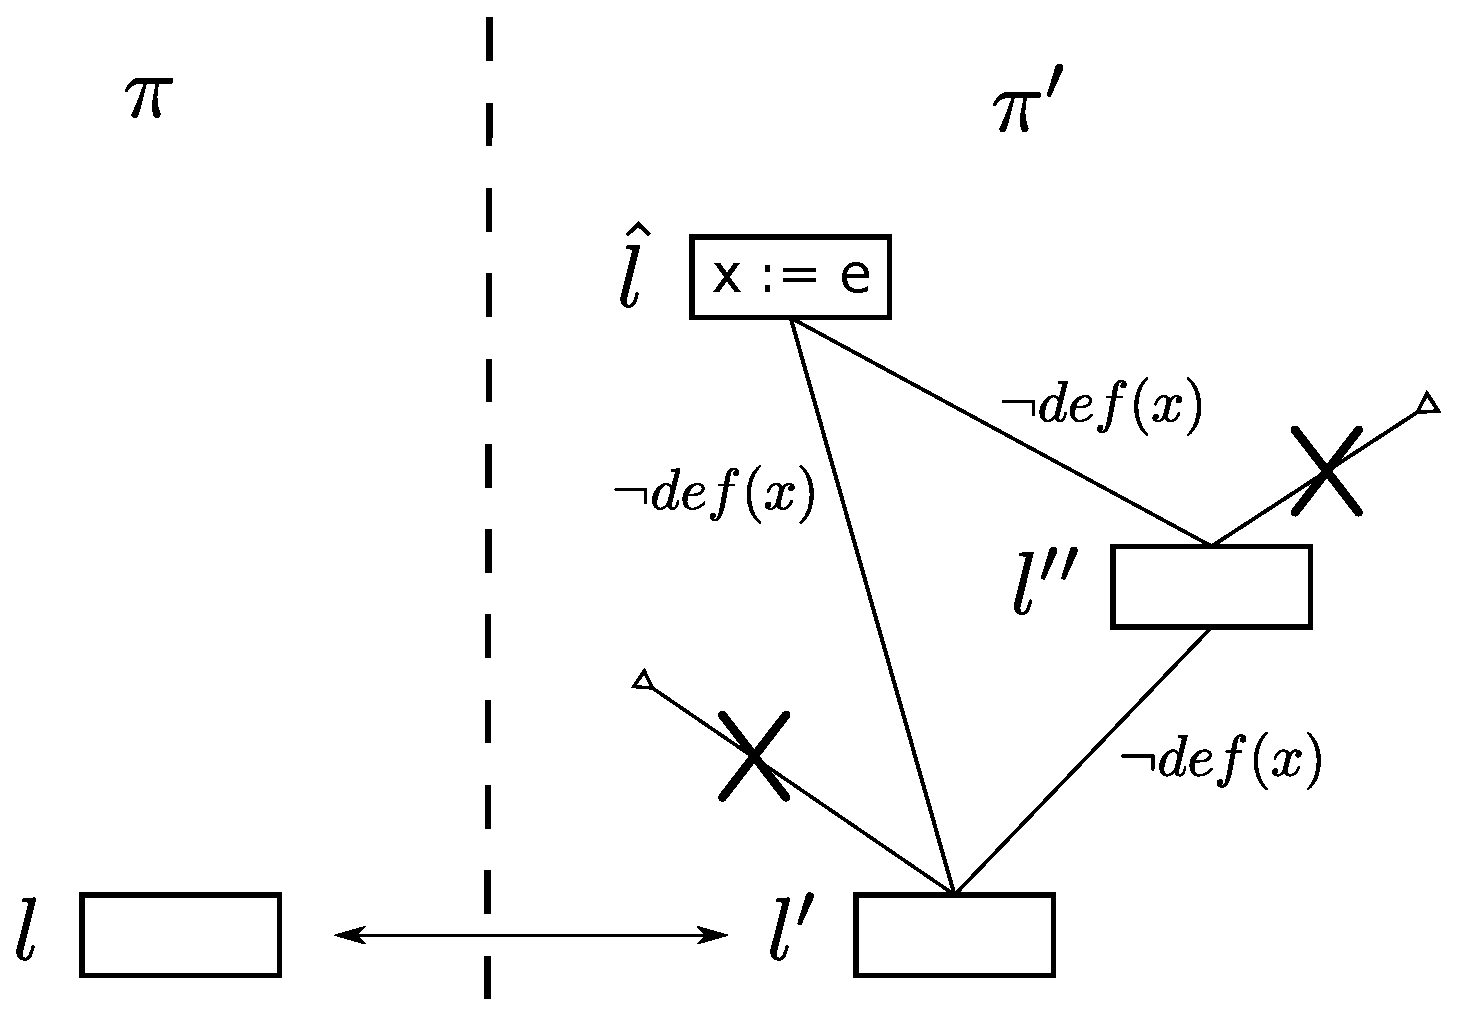
\includegraphics[width=0.49\textwidth]{figures/osr-reconstruct/osr-reconstruct.eps}
\caption{\protect\label{fig:osr-reconstruct} Algorithm \reconstruct\ identifies an assignment \mytt{x:=e} at $\hat{l}$ that reaches both $l'$ and $l''$, and no other definition of \wx\ is possible.}
\end{center}
\end{figure}
\fi

\begin{definition}[Live-Variable Equivalent Transformation]
\label{de:lve-trans}
A program transformation $T$ is {\em live-variable equivalent} (LVE) if for any program $\pi$, $\pi$ and $\mysem{T}(\pi)$ are live-variable bisimilar.
\end{definition}

\noindent We can finally establish the correctness of ${\tt OSR\_trans}$, which follows directly by \Cref{le:lvb-same-loc,le:build-comp-corr} and \ref{co:same-size}:

\begin{theorem}
\label{th:osr-trans-correctness}
For any program $\pi$ and live-variable equivalent transformation $T$, if ${\tt apply}(\pi,T)\triangleq(\pi', \Delta_I, \Delta_I)$ where $\pi'=\mysem{T}(\pi)$ and $\Delta_I:[1,|\pi|]\rightarrow [1,|\pi|]$ is the identity mapping between program points, then ${\tt OSR\_trans}(\pi,T)$ $=(\pi',\mu_{\pi\pi'},\mu_{\pi'\pi})$ yields a strict OSR mapping $\mu_{\pi\pi'}$ between $\pi$ and $\pi'$ and a strict OSR mapping $\mu_{\pi'\pi}$ between $\pi'$ and $\pi$.
\end{theorem}

\paragraph*{Discussion.} We remark that the assumption of an identity mapping between program points, which is a necessary condition of live-variable bisimilarity, is without loss of generality as it can  always be enforced by padding programs with \wskip\ statements. For instance, the Hoist transformation of \myfigure\ref{fig:sample-trans}, which we prove to be LVE in the next section, replaces the hoisted instruction with a \wskip, and expects a \wskip\ to already exist at the point where it is moved. As we discuss in \mysection\ref{ss:BC-implementation}, this is not required in a real compiler, as a transformation pass can be instrumented to capture code modifications that require updating the mapping.

\subsubsection{Examples of LVE Transformations}

\label{ss:lve-trans}

In this section, we show that classic compiler optimizations such as constant propagation, dead code elimination, and code hoisting as defined in \myfigure\ref{fig:sample-trans} are all examples of live-variable equivalent transformations. Hence, they are provably correct building blocks of an OSR-aware compilation toolchain based on algorithm $\osrtrans$. These optimizations are representatives of a broad class of transformations that insert, delete, and modify instructions. Further optimizations, which we do not formally discuss in this paper, are evaluated in \missing.

\begin{theorem}
\label{th:lve-trans-examples}
Transformations CP, DCE, and Hoist of \myfigure\ref{fig:sample-trans} are live-variable equivalent.
\end{theorem}

\begin{myproof}
\missing
In \cite{Lacey04}, CP, DCE, and Hoist are proven correct, each using a different bisimulation relation $R$. We propose a unifying approach based on live-variable bisimilarity. Let $\theta$ be a substitution that bounds free meta-variables with concrete program objects so that a rule's side-condition is satisfied. For CP, $R$ is the identity relation, hence $A(l)=Val\supseteq \live(\pi,l)\cap \live(\pi',l)$ in \mydefinition\ref{de:state-equiv-relation}. In DCE, $R$ is the identity relation before the eliminated assignment \mytt{x:=e}, and $A(l)=Val\setminus\{\theta(\wx)\}=\live(\pi,l)\cap \live(\pi',l)$ after it. For Hoist, $R$ is the identity relation before $\theta(p)$ and after $\theta(q)$ (see \myfigure\ref{fig:sample-trans}), and $A(l)=Val\setminus\{\theta(\wx)\}=\live(\pi,l)\cap \live(\pi',l)$ between them.
\end{myproof}
% !TEX root = thesis.tex

\subsubsection{Composing Multiple Transformation Passes}
\label{ss:trans-compose}

In this section, we show that OSR mappings can be composed, allowing several optimization passes to be applied to a program using algorithm ${\tt OSR\_trans}$. The first ingredient is {\em program composition}, defined as follows:

\begin{definition}[Program composition]
\label{de:composition}
We say that two programs $\pi,\pi'\in Prog$ with $\pi=\langle I_1,\ldots,I_n\rangle$ and $\pi'=\langle I'_1,\ldots,I'_{n'}\rangle$ are {\em composable} if $I_n=\texttt{out}~v_1,\ldots,v_k$ and $I'_1=\texttt{in}~v'_1,\ldots,v'_{k'}$ with $\{v'_1,\ldots,v'_{k'}\}\subseteq\{v_1,\ldots,v_k\}$. For any pair of composable programs $\pi,\pi'$, we define $\pi\circ\pi'=\langle I_1,\ldots,I_{n-1},\hat{I'}_2,\ldots,\hat{I'}_{n'}\rangle$, where $\forall i\in[1,n']$, $\hat{I'}_i$ is obtained from $I'_i$ by relocating each {\tt goto} target $m$ with $m+n-2$.
\iffalse
where $\chi\circ\chi'=\chi\setminus\{{\tt out \ldots}\}\cdot\chi'\left[
\begin{tiny}
\begin{array}{l}
\texttt{goto}~m\mapsto \\
\texttt{goto}~m+|\chi|-2
\end{array}
\end{tiny}
\right]\setminus\{{\tt in \ldots}\}$. 
\fi
\end{definition}

\begin{lemma}[Semantics of program composition]
\label{le:prog-comp-sem}
Let $\pi,\pi'\in Prog$ be any pair of composable programs, then $\forall\sigma\in\Sigma,$ $\mysem{\pi\circ\pi'}(\sigma)=\mysem{\pi'}\left(\mysem{\pi}(\sigma)\right)$.
\end{lemma}
\begin{myproof}
Straightforward by~\Cref{de:program-semantics,de:composition}.
\end{myproof}

\noindent We show how to define a composition of OSR mappings and we prove that it yields a valid OSR mapping.

\begin{lemma}[Mapping Composition]
\label{le:osr-mapping-comp}
Let $\pi,\pi',\pi''\in Prog$, let $\mu_{\pi\pi'}$ and $\mu_{\pi'\pi''}$ be OSR mappings as in \mydefinition\ref{de:osr-mapping}, and let $\mu_{\pi\pi'}\circ\mu_{\pi'\pi''}$ be a {\em composition of mappings} defined as follows:
\begin{gather*}
\forall l\in dom(\mu_{\pi\pi'})~s.t.~\mu_{\pi\pi'}(l)=(l',\chi)\wedge l'\in dom(\mu_{\pi'\pi''}):\\
\mu_{\pi'\pi''}(l')=(l'',\chi')\implies(\mu_{\pi\pi'}\circ\mu_{\pi'\pi''})(l)=(l'',\chi\circ\chi')
\end{gather*}
Then $\mu_{\pi\pi'}\circ\mu_{\pi'\pi''}$ is an OSR mapping from $\pi$ to $\pi''$.
\end{lemma}

\begin{myproof} 
Let $\mu_{\pi\pi''}=\mu_{\pi\pi'}\circ\mu_{\pi'\pi''}$. By \mydefinition\ref{de:osr-mapping}, it holds:
\begin{small}
\begin{gather*}
\forall \sigma\in\Sigma, \forall s_i=(\sigma_i,l_i)\in\tau_{\pi\sigma}~\text{s.t.}~l_i\in dom(\mu_{\pi\pi''}),\\
\exists \sigma',\sigma''\in\Sigma,~\exists s_j=(\sigma_j,l_j)\in\tau_{\pi'\sigma'}, \\ \exists s_k=(\sigma_k,l_k)\in\tau_{\pi''\sigma''}~\text{s.t.}~
\mu_{\pi\pi''}(l_i)=(l_k,\chi\circ\chi')~\wedge~\\ \mysem{\chi\circ\chi'}(\sigma_i\vert_{\live(\pi,l_i)})=\text{[by \ref{le:prog-comp-sem}]}\\
\mysem{\chi'}(\mysem{\chi}(\sigma_i\vert_{\live(\pi,l_i)}))=
\mysem{\chi'}(\sigma_j\vert_{\live(\pi',l_j)})=\sigma_k\vert_{\live(\pi'',l_k)}
\end{gather*}
\end{small}
\noindent Hence, $\mu_{\pi\pi'}\circ\mu_{\pi'\pi''}$ is an OSR mapping from $\pi$ to $\pi''$.
\end{myproof}

\begin{corollary}
\label{co:compose-strict}
Let $\pi,\pi',\pi''\in Prog$, let $\mu_{\pi\pi'}$ and $\mu_{\pi'\pi''}$ be strict OSR mappings as in \mydefinition\ref{de:osr-mapping}. Then $\mu_{\pi\pi'}\circ\mu_{\pi'\pi''}$ is a strict OSR mapping from $\pi$ to $\pi''$.
\end{corollary}
\begin{myproof}
Straightforward by \mydefinition\ref{de:osr-mapping} and \ref{le:osr-mapping-comp}.
\end{myproof}

\ifdefined\noauthorea
\begin{figure}[ht!]
\IncMargin{2em}
\begin{algorithm}[H]
\DontPrintSemicolon
\LinesNumbered
\SetAlgoNoLine
\SetNlSkip{1em} 
\Indm\Indmm
\hrulefill\\
\KwIn{Program $\pi$, list of program transformations $L$.}
\KwOut{Program $\hat{\pi}$, mappings $\mu_{\pi\hat{\pi}}$ and $\mu_{\hat{\pi}\pi}$.}
\nonl\vspace{-2mm}\hrulefill\\
\nonl$\mathbf{algorithm} \> \> \dopasses$($\pi$, $T::L$)$\rightarrow$($\pi''$, $\mu_{\pi\pi''}$, $\mu_{\pi''\pi}$):\;
\everypar={\nl}
\Indp\Indpp
\vspace{1mm} $(\pi',\mu_{\pi\pi'},\mu_{\pi'\pi})\gets \osrtrans(\pi,T)$\;
\lIf{$L=Nil$}{
    \Return{$(\pi',\mu_{\pi\pi'},\mu_{\pi'\pi})$}
}
$(\pi'',\mu_{\pi'\pi''},\mu_{\pi''\pi'})\gets \dopasses(\pi',L)$\;
\Return{$(\pi'',\mu_{\pi\pi'}\circ\mu_{\pi'\pi''},\mu_{\pi''\pi'}\circ\mu_{\pi'\pi})$}\;
\vspace{-2mm}
\Indm\Indmm
\nonl\hrulefill\vspace{1mm}\\
\DecMargin{2.5em}
\caption{\label{alg:osr-trans-compose} OSR-aware multi-pass program transformations.}
\IncMargin{2.5em}
\end{algorithm} 
\end{figure}

\else
\begin{figure}
\noindent
\begin{small}
\hphantom{xxx} $\textbf{algorithm}~{\tt do\_passes}(\pi, T::L)\rightarrow (\pi'',\mu_{\pi\pi''},\mu_{\pi''\pi})$ \\
1. ~~ ~~~~ $(\pi',\mu_{\pi\pi'},\mu_{\pi'\pi})\gets {\tt OSR\_trans}(\pi,T)$ \\
2. ~~ ~~~~ $\textbf{if}~L=Nil~\textbf{return}~ (\pi',\mu_{\pi\pi'},\mu_{\pi'\pi})$ \\
3. ~~ ~~~~ $(\pi'',\mu_{\pi'\pi''},\mu_{\pi''\pi'})\gets {\tt do\_passes}(\pi',L)$ \\
4. ~~ ~~~~ $\textbf{return}~(\pi'',\mu_{\pi\pi'}\circ\mu_{\pi'\pi''},\mu_{\pi''\pi'}\circ\mu_{\pi'\pi})$ \\
\end{small}
\caption{OSR-aware multi-pass program transformations.}
\label{alg:osr-trans-compose}
\end{figure}
\fi

\noindent Based on \ref{le:osr-mapping-comp}, we can easily prove by induction the correctness of the multi-pass transformation algorithm of \myalgorithm\ref{alg:osr-trans-compose}, which takes a program $\pi$ and a list of program transformations, and applies them to $\pi$, producing a bidirectional OSR mapping $\mu_{\pi\pi''},\mu_{\pi''\pi}$ between $\pi$ and the resulting program $\pi''$.
\subsection{Multi-Version Programs}

In this section, we propose a general OSR model where computations are described by a {\em multi-version program}, which consists of different versions of a program along with OSR mappings that allow execution to be transferred between them.

\begin{definition}[Multi-Version Program]
\label{de:mv-program}
A multi-version program is modeled by an edge-labeled graph $\Pi=({\cal V}, {\cal E}, {\cal M})$ where ${\cal V}=\{ \pi_1, \pi_2, \ldots,\pi_r\}$ is a set of program versions, ${\cal E}\subseteq \Pi^2$ is a set of edges such that $(\pi_p,\pi_q)$ indicates that an OSR transition can be fired from some point of $\pi_p$ to $\pi_q$,
%any point in $dom({\cal M}(\pi_i,\pi_j))$, 
and ${\cal M}:{\cal E}\rightarrow OSRMap$ labels each edge $(\pi,\pi')\in {\cal E}$ with an OSR mapping from $\pi$ to $\pi'$.
\end{definition}

\subsubsection*{Semantics}

The state of a multi-version program is similar to the state of a program (\ref{de:prog-state}), but it also includes the index of the currently executed program version:

\begin{definition}[Multi-Version Program State]
The {\em state} of a multi-version program $\Pi=({\cal V}, {\cal E}, {\cal M})$ is described by a triple $(p,\sigma,l)$, where $p\in[1,|{\cal V}|]$ is the index of a program version, $\sigma$ is a memory store, and $l\in [1,|\pi_p|]$ is the point of the next instruction to be executed in $\pi_p$. The {\em initial state} from a store $\sigma$ is $(1,\sigma,1)$, i.e., computations start at $\pi_1$. We denote by $MState=\mathbb{N}\times\Sigma\times \mathbb{N}$ the set of all possible multi-version program states.
\end{definition}

\noindent The execution semantics of a multi-version program is described by the following transition relation:

\begin{definition}[Multi-Version Big-Step Transitions]
\label{de:osr-semantics}
For any multi-version program $\Pi$, relation $\Rightarrow_{\Pi}\subseteq MState\times MState$ is defined as follows:%, with meta-variables $\texttt{x}, \texttt{y}\in Var$, $\texttt{e}\in Expr$, and $\texttt{m}\in Num$:

\begin{footnotesize}
\begin{equation}
\label{eq:mv-big-step}
\begin{array}{rc}
(Norm)
&
\dfrac
{(\sigma, l)\Rightarrow_{\pi_p} (\sigma',l')}
{(p,\sigma, l)\Rightarrow_{\Pi} (p,\sigma',l')}
\\
\\
(OSR)
&
\dfrac
{(\pi_p,\pi_q)\in {\cal E} ~ \wedge ~ (l',\chi)={\cal M}(\pi_p,\pi_q)(l) ~ \wedge ~ \sigma'=\mysem{\chi}(\sigma)}
{(p,\sigma, l)\Rightarrow_{\Pi} (q,\sigma',l')}\\
\end{array}
\end{equation}
\end{footnotesize}
\end{definition}

\noindent The meaning is that at any time, execution can either continue in the current program version (Norm rule), or an OSR transition -- if possible at the current point -- can direct the control to another program version (OSR rule). The choice is non-deterministic, i.e., an oracle can tell the execution engine which rule to apply. In practice, the choice may be based for instance on profile data gathered by the runtime system: a common strategy is to dynamically ``OSR'' to the available version with the best expected performance on the actual workload. Notice that since $\Rightarrow_{\Pi}$ may be non-deterministic, in general there may be different final stores for the same initial store. However, we are only interested in multi-version programs that deterministically yield a unique result, which guarantees semantic transparency of OSR transitions. 

To characterize the execution behavior of a multi-version program, we consider the system of traces of an execution transition system that start from a given initial state.

\begin{definition}[Trace System of Multi-Version Program]
\label{de:mvp-exec-system}
The system of traces ${\cal T}_{\Pi,\sigma}$ contains all traces $\tau$ of transition system $(MState,\Rightarrow_{\Pi})$ such that $\tau[0]=(1,\sigma,1)$.
\end{definition}

\begin{definition}[Deterministic Multi-Version Program]
\label{de:deterministic-mvp}
A multi-version program $\Pi$ is deterministic iff $\forall \sigma\in\Sigma$, either all traces in ${\cal T}_{\Pi,\sigma}$ are infinite, or they all lead to the same store, i.e.:
\begin{gather*}
\forall \tau, \tau'\in{\cal T}_{\Pi,\sigma}: ~~ \big(|\tau|=\infty ~ \Longleftrightarrow ~ |\tau'|=\infty\big) ~ \wedge \\
\big(|\tau|<\infty ~ \Longrightarrow ~ \exists~p,p',l,l'\in\mathbb{N}, \sigma,\sigma'\in\Sigma: ~ \\
\tau[|\tau|]=(p,\sigma,l) ~ \wedge ~ \tau'[|\tau'|]=(p',\sigma',l') ~ \wedge ~ \sigma=\sigma' \big).
\end{gather*}
\end{definition}

\noindent The meaning of a deterministic multi-version program can be defined as follows:

\begin{definition}[Multi-Version Semantic Function]
\label{de:mv-program-semantics}
The semantic function $\mysem{\Pi}:\Sigma \rightarrow \Sigma$ of a deterministic multi-version program $\Pi$ is defined as: 
$$
%\forall \sigma\in\Sigma: ~~ \mysem{\Pi}(\sigma)=\sigma' ~~ \Longleftrightarrow ~~ (1,\sigma,1) \Rightarrow^{*}_{\Pi} (p,\sigma',|\pi_p|+1) ~ \}
\forall \sigma\in\Sigma: ~~ \mysem{\Pi}(\sigma)=\sigma' ~~ \Longleftrightarrow ~~ (1,\sigma,1) \Rightarrow^{*}_{\Pi} (p,\sigma',|\pi_p|+1)
$$
where $\Rightarrow^{*}_{\Pi}$ is the transitive closure of $\Rightarrow_{\Pi}$.
\end{definition}

\subsubsection*{Generation Algorithm and Correctness}

A natural way to generate a multi-version program consists in starting from a base program $\pi_1$ and constructing a tree of different versions, where each version is derived from its parent by applying one or more transformations. Using this approach and procedure \dopasses\ described in \mysection\ref{ss:trans-compose}, it is straightforward to construct a multi-version program $\Pi=({\cal V}, {\cal E}, {\cal M})$ such that:
\vspace{-1mm}
\begin{align*}
(\pi_p,\pi_q)\in {\cal E} ~~ \Longleftrightarrow ~~ \exists L: ~ &{\tt do\_passes}(\pi_p,L)=(\pi_q,\mu,\mu') ~ \wedge ~ {\cal M}(\pi_p,\pi_q)=\mu ~~ \vee \\
&{\tt do\_passes}(\pi_q,L)=(\pi_p,\mu,\mu') ~ \wedge ~ {\cal M}(\pi_p,\pi_q)=\mu'
\end{align*}

\noindent To prove the correctness of this approach, we introduce a preliminary lemma and then use it to prove that a multi-version program built in this way is deterministic.

\begin{lemma}
\label{le:comp-lemma}
Let $\tau\in{\cal T}_{\Pi,\sigma}$ be an execution trace in the system of the traces for the multi-version program $\Pi$ $=({\cal V}, {\cal E}, {\cal M})$ constructed using \dopasses\ and LVE transformations, and let $\omega_1,\ldots,\omega_k$ be the indices of $\tau$ where an OSR transition has just occurred, with $\tau[\omega_i]=(p_{\omega_i}, \sigma_{\omega_i}, l_{\omega_i})$. Then $\forall i\in[1,k]$ there exists a state $(\hat{\sigma}_i,\hat{l}_i)$ in the trace of $\pi_{p_{\omega_{i}}}$ starting from the initial store $\sigma$ such that $\hat{l}_i=l_{\omega_i}$ and $\hat{\sigma}_i\vert_{\live(\pi_{p_{\omega_{i}}},\,\hat{l}_i)}=\sigma_{\omega_i}\vert_{\live(\pi_{p_{\omega_{i}}},\,\hat{l}_i)}$.
\end{lemma}
\begin{myproof}
To simplify the notation we introduce:
\begin{equation*}
\hat{\pi}_i = \begin{cases}
\pi_1 & \text{if } i=0\\
\pi_{p_{\omega_i}} & \text{if } i \in [1,k]
\end{cases}
\end{equation*}

\noindent From \ref{eq:mv-big-step} we can write that $\tau[\omega_i]=(p_{\omega_i}, \sigma_{\omega_i},l_{\omega_i})$ has been obtained from $\tau[\omega_i-1]=(p_{\omega_i-1}, \sigma_{\omega_i-1}, l_{\omega_i-1})$ with $\sigma_{\omega_i}=\mysem{\chi_{\omega_i-1}}(\sigma_{\omega_i})$. For each OSR transition $\hat{\pi}_i$ has been obtained from $\hat{\pi}_{i-1}$ using \dopasses\ for some sequence $L$ of LVE transformations. Indeed, in order for \ref{eq:mv-big-step} to apply:
\begin{align*}
(\hat{\pi}_{i-1},\hat{\pi}_i)\in{\cal E} ~\wedge~ \exists L: ~&{\tt do\_passes}(\hat{\pi}_{i-1}, L-1)=(\hat{\pi}_i,\mu_{\hat{\pi}_{i-1}\hat{\pi}_i},{\mu'}_{\hat{\pi}_{i}\hat{\pi}_{i-1}}) ~\wedge~\\
&M(\hat{\pi}_{i-1},\hat{\pi}_i)=\mu_{\hat{\pi}_{i-1}\hat{\pi}_i}
\end{align*}

\noindent When the OSR step is performed we thus have:
\begin{equation*}
M(\hat{\pi}_{i-1},\hat{\pi}_i)(l_{\omega_i-1})=\mu_{\hat{\pi}_{i-1}\hat{\pi}_i}(l_{\omega_i-1})=(l_{\omega_i},\chi_{\omega_i-1})
\end{equation*}

\noindent By \ref{th:osr-trans-correctness} function $\mu_{\hat{\pi}_{i-1}\hat{\pi}_i}$ provides a strict OSR mapping between $\hat{\pi}_{i-1}$ and $\hat{\pi}_i$, as all LVE transformations in L are composed into a strict mapping (\ref{co:compose-strict}). Note also that since $\Delta_I$ is being used to map OSR program points between $\hat{\pi}_{i-1}$ and $\hat{\pi}_i$, it follows that $l_{\omega_i}=l_{\omega_i-1}~\forall i\in[1,k]$.
We now prove our claim by induction on $i$.

\paragraph*{Base step.} When $i=1$, we know that no OSR transition has been performed till $l_{\omega_1-1}$ and $\hat{\pi}_0$ has been executing all the time. Then we can write:
\begin{equation*}
(1, \sigma, 1)\trans^*_{\Pi}(1,\sigma_{\omega_1-1},l_{\omega_1-1}) \Longleftrightarrow (\sigma, 1) \trans^*_{\hat{\pi}_0} (\sigma_{\omega_1-1},l_{\omega_1-1})
\end{equation*}

\noindent Trivially, $(\sigma_{\omega_1-1},l_{\omega_1-1})\in\tau_{\hat{\pi}_0\sigma}$. We can thus infer from \ref{de:osr-mapping}:
\begin{align*}
\exists s_j=(\sigma_j,l_j)\in\tau_{\hat{\pi}_1\sigma}~\text{s.t.}~&\mu_{\hat{\pi}_{0}\hat{\pi}_1}(l_{\omega_1-1})=(l_j,\chi)~\wedge \\
&\mysem{\chi}(\sigma_{\omega_1-1}\vert_{\live(\hat{\pi}_{0},\,l_{\omega_1-1})})=\sigma_j\vert_{\live(\hat{\pi}_{1},\,l_j)}
\end{align*}

\noindent From the definition of $\mu_{\hat{\pi}_{0}\hat{\pi}_1}$ it follows that $\chi=\chi_{\omega_1-1}$ and $l_j=l_{\omega_1}=l_{\omega_1-1}$. To prove the claim we need to show that:

\begin{equation*}
\sigma_j\vert_{\live(\hat{\pi}_{1},\,l_{\omega_1})}=\sigma_{\omega_1}\vert_{\live(\hat{\pi}_{1},\,l_{\omega_1})}
\end{equation*}

\noindent which follows directly from \Cref{le:build-comp-corr,le:osr-mapping-comp}.

\paragraph*{Inductive step.} As inductive hypothesis we assume that $\exists (\hat{\sigma}_{k-1},\hat{l}_{k-1})\in\tau_{\hat{\pi}_{k-1}\sigma}$ s.t.:
\begin{equation*}
\hat{l}_{k-1}=l_{\omega_{k-1}} ~\wedge~ \hat{\sigma}_{k-1}\vert_{\live(\hat{\pi}_{k-1},\,\hat{l}_{k-1})}=\sigma_{\omega_{k-1}}\vert_{\live(\hat{\pi}_{k-1},\,\hat{l}_{k-1})}
\end{equation*}

\noindent
Since no OSR is performed between $\tau[\omega_{k-1}]$ and $\tau[\omega_k-1]$ we can write:
\begin{gather*}
(\hat{\sigma}_{k-1}, l_{\omega_{k-1}}) \trans^*_{\hat{\pi}_{k-1}} \cdots \trans^*_{\hat{\pi}_{k-1}} (\tilde{\sigma},l_{\omega_k-1}) \Longleftrightarrow \\
(\sigma_{\omega_{k-1}}, l_{\omega_{k-1}}) \trans^*_{\hat{\pi}_{k-1}} \cdots \trans^*_{\hat{\pi}_{k-1}} (\sigma_{\omega_k-1},l_{\omega_k-1})
\end{gather*}

\noindent in the same number of steps, with $\tilde{\sigma}\vert_{\live(\hat{\pi}_{k-1},\,l_{\omega_k-1})} = \sigma_{\omega_k-1}\vert_{\live(\hat{\pi}_{k-1},\,l_{\omega_k-1})}$ by \ref{le:only-live-count}. Since $(\tilde{\sigma},l_{\omega_k-1})\in\tau_{\hat{\pi}_{k-1}\sigma}$ by the strictness of the OSR mapping $\mu_{\hat{\pi}_{k-1}\hat{\pi}_{k}}$:
\begin{align*}
\exists s_j=(\sigma_j,l_j)\in\tau_{\hat{\pi}_k\sigma}~\text{s.t.}~&\mu_{\hat{\pi}_{k-1}\hat{\pi}_{k}}(l_{\omega_k-1})=(l_j,\chi)~\wedge \\
&\mysem{\chi}(\tilde{\sigma}\vert_{\live(\hat{\pi}_{k-1},\,l_{\omega_k-1})})=\sigma_j\vert_{\live(\hat{\pi}_{k},\,l_j)}
\end{align*}

\noindent From the definition of $\mu_{\hat{\pi}_{k-1}\hat{\pi}_k}$ it follows that $\chi=\chi_{\omega_k-1}$ and $l_j=l_{\omega_k}=l_{\omega_k-1}$. By \Cref{le:build-comp-corr,le:osr-mapping-comp} we thus prove:
\begin{align*}
\sigma_j\vert_{\live(\hat{\pi}_{k},\,l_{\omega_k})} &= \mysem{\chi_{\omega_k-1}}(\tilde{\sigma}\vert_{\live(\hat{\pi}_{k-1},\,l_{\omega_k-1})})\\
&=\mysem{\chi_{\omega_k-1}}(\sigma_{\omega_k-1}\vert_{\live(\hat{\pi}_{k-1},\,l_{\omega_k-1})})\\
&=\sigma_k\vert_{\live(\hat{\pi}_{k},\,l_{\omega_k})})
\end{align*}
\end{myproof}

\begin{theorem}[Multi-Version Program Determinism]
\label{th:mv-prog-determ}
Let $\Pi$ $=({\cal V}, {\cal E}, {\cal M})$ be a multi-version program constructed using \dopasses\ and live-variable equivalent transformations. Then $\Pi$ is deterministic.
\end{theorem}

\begin{myproof}
To prove that $\Pi$ is deterministic, we need to show that, given any initial store $\sigma$ on which $\pi_1\in\Pi$ terminates on some final state $\sigma'=\mysem{\pi_1}(\sigma)$, any execution trace $\tau\in{\cal T}_{\Pi,\sigma}$ terminates with $\sigma'$.

Let $\omega_1,\ldots,\omega_k$ be the indices of $\tau$ where an OSR transition has just occurred, i.e., for any $i\in[1,k]$, state $\tau[\omega_i]$ is obtained from $\tau[\omega_i-1]$ by applying compensation code $\chi_{\omega_i-1}$ on store $\sigma_{\omega_i-1}$, which yields a store $\sigma_{\omega_i}$. The transition leads from a point $l_{\omega_i-1}$ in version $\pi_{p_{\omega_i-1}}$ to a point $l_{\omega_i}=l_{\omega_i-1}$ in version $\pi_{p_{\omega_{i}}}$ in $\Pi$. 

By \mylemma\ref{le:comp-lemma}, $\forall i\in[1,k]$ there exists a state $(\hat{\sigma}_i,\hat{l}_i)$ in the trace of $\hat{\pi}_i=\pi_{p_{\omega_{i}}}$ starting from the initial store $\sigma$ such that $\hat{l}_i=l_{\omega_i}$ and $\hat{\sigma}_i\vert_{\live(\hat{\pi}_i,\hat{l}_i)}=\sigma_{\omega_i}\vert_{\live(\hat{\pi}_i,\hat{l}_i)}$. Hence, since no OSR is fired after $\omega_k$, by \myequation\ref{eq:mv-big-step} it holds: 
\begin{equation*}
(\hat{\pi}_k,\sigma_{\omega_{k}},l_{\omega_{k}})\trans^*_{\Pi}(\hat{\pi}_k,\sigma',|\hat{\pi}_k|+1) \Longleftrightarrow (\sigma_{\omega_{k}},l_{\omega_{k}})\trans^*_{\hat{\pi}_k}(\sigma',|\hat{\pi}_k|+1)
\end{equation*}

\noindent We can then apply \Cref{le:only-live-count,le:comp-lemma} to write:
\begin{gather*}
(\sigma_{\omega_{k}},l_{\omega_{k}})\trans^*_{\hat{\pi}_k}(\sigma',|\hat{\pi}_k|+1) \Longleftrightarrow \\ 
(\sigma_{\omega_{k}}\vert_{\live(\hat{\pi}_k,l_{\omega_{k}})},l_{\omega_{k}})\trans^*_{\hat{\pi}_k}(\sigma',|\hat{\pi}_k|+1) \Longleftrightarrow \\
(\hat{\sigma}_k\vert_{\live(\hat{\pi}_k,\hat{l}_k)},\hat{l}_k)\trans^*_{\hat{\pi}_k}(\sigma',|\hat{\pi}_k|+1)
\end{gather*}

\noindent As $(\hat{\sigma}_k,\hat{l}_k)\in\tau_{\hat{\pi}_k\sigma}$, by \ref{le:only-live-count} necessarily $\sigma'=\mysem{\hat{\pi}_k}(\sigma)$. 
Given that all programs in $\Pi$ are semantically equivalent, we can conclude that $\mysem{\Pi}(\sigma)=\sigma'=\mysem{\hat{\pi}_k}(\sigma)=\mysem{\pi_1}(\sigma)$.
\end{myproof}




\subsection{Discussion}
The techniques described in the previous pages represent a first step towards a provably sound methodological framework for on-stack replacement. OSR is not only a great engineering problem, but also an intellectually challenging endeavor. We think that our formalization, by distilling OSR to an abstract program morphing problem, may help to prototype better continuous optimizations.

A key innovation we introduce is the ability to make single passes OSR-aware in isolation, and then flexibly combine them in any order by exploiting the composability of the glue code. Think for instance of applying a speculative optimization (e.g., aggressive inlining in a dynamic language), followed by further passes enabled by that optimization. Without a principled approach to composing glue code, dynamically jumping to a safe version by undoing all the applied optimizations when an assumption fails becomes a daunting engineering task that only production runtimes such as HotSpot dare to pursue. Demystifying OSR can allow the community to contribute.

Ideally, the presence of an OSR point should be completely transparent, without slowing down the performance of the code in any way. However, this may not always be possible as a glue code may require state portions to be logged during the program's execution. Our work lies at the performance-preserving end of the spectrum, as we do not impose any barriers to optimizations, which run unhindered, and we do not require any state logging. We assess the practical impact of this design choice in \mysection\ref{se:eval-OSR-alC}, in which we experimentally analyze in prominent benchmarks the fraction of program locations where OSR can be efficiently fired in the presence of several optimization passes from the LLVM compiler toolchain.

%we present promising results on real benchmarks to which extent glue code can be generated by only relying on the live state at the OSR origin.
%There is a trade-off between the number of points where OSR can be correctly fired and the price to pay in terms of space and time in order to support them. Our work lies at the performance-preserving end of the spectrum, supporting OSR transitions in constant time and space. The approach we propose does not impose any barriers to optimizations, which run unhindered, and does not require any state logging. To assess the practical impact of this design choice, in \mysection\ref{se:evaluation} we analyze experimentally on prominent benchmarks - and across several optimization passes in the LLVM compiler toolchain - to which extent glue code can be generated by only relying on the live state at the OSR origin.

A deep understanding of OSR's flexibility/performance trade-offs remains nonetheless a compelling goal. How can we perform fine-grained OSR transitions across transformations that significantly change the structure of a program, as aggressive loop optimizations do? How can we handle situations where the landing location of an OSR transition may not be unique, as in software pipelining~\cite{Kundu09}? We probably open more questions than we solve.

\subsection{Comparison with Related Work}
In this section we discuss the connections of our ideas with previous works. For existing OSR implementations - in which the generation of compensation code is left to code optimizers - we refer the reader to \mysection\ref{ss:osr-llvm-related}.

\paragraph*{Correctness of Compiler Optimizations.} Translation validation~\cite{Pnueli98, Necula00} tackles the problem of verifying that the optimized version of a specific input program is semantically equivalent to the original program. Lacey et al.~\cite{Lacey02, Lacey04} propose to express optimizations as rewrite rules with CTL formulas as side conditions, showing how to prove such transformations correct. \cite{Lerner03, Lerner05, Kundu09} investigate how to automatically prove soundness for optimizations expressed in terms of transformation rules. In particular, a further step towards generality is made in~\cite{Kundu09}: proving the equivalence of {\em parameterized programs} enables proving the correctness of transformation rules once for all. We believe that this approach deserves further investigation in the OSR context, as it could provide a principled approach to computing mappings between equivalent points in different program versions in the presence of complex optimizations. 

While all the aforementioned works focus on proving optimizations sound, in this thesis we aim at proving OSR correct in the presence of optimizations. Of a different flavor, but in a similar spirit as ours, Guo and Palsberg~\cite{Guo11} use bisimulation to study what optimizations of a tracing JIT compiler are sound. OSR is used in traditional JIT compilation to devise efficient code for a whole method, while a tracing JIT performs aggressive optimizations on a linear sequence of instructions, which may return from guarded side exits when the control flow diverges from the recorded trace.

\paragraph*{Debugging Optimized Code.} Hennessy's seminal paper~\cite{Hennessy82} has sparked a lot of interest in debugging of optimized code in the past three decades (e.g., ~\cite{Coutant88, Adl-Tabatabai96, Wu99, Jaramillo00, Barr14}). Some works~\cite{Hennessy82, Wu99} in particular attempt to reconstruct source-level variable values in the presence of certain optimizations. We discuss our connections with them in \mysection\ref{se:CS-debug}, in which we explore the end-to-end utility of our OSR mappings in the context of a source-level debugger.

\paragraph*{Other Related Work.} Program slicing techniques~\cite{Weiser82,Weiser84, Korel88, Agrawal90} have found many diverse applications, such as program debugging, comprehension, analysis, testing, verification and optimization. Given a slicing criterion consisting of a program point P and several variables used at P, program slicing computes a slice of the program that may affect their values at P in terms of data and control dependences~\cite{Tan16}. We believe that the simple ideas behind our \buildcomp\ algorithm could be improved by taking advantage of this wealth of analysis techniques.

Another interesting work to look at is~\cite{Bhandari15}, which explores deoptimization in the presence of exceptions for the loop tiling transformation. In order to be able to rollback out-of-order updates, an algorithm identifies a minimal number of elements to backup and generates the necessary code. Intuitively, supporting deoptimization for complex loop transformations may be both space- and time- costly, but in the OSR context flexibility/performance trade-offs are still largely unexplored.